% Options for packages loaded elsewhere
\PassOptionsToPackage{unicode}{hyperref}
\PassOptionsToPackage{hyphens}{url}
%
\documentclass[
  11pt,
]{article}
\usepackage{lmodern}
\usepackage{amsmath}
\usepackage{ifxetex,ifluatex}
\ifnum 0\ifxetex 1\fi\ifluatex 1\fi=0 % if pdftex
  \usepackage[T1]{fontenc}
  \usepackage[utf8]{inputenc}
  \usepackage{textcomp} % provide euro and other symbols
  \usepackage{amssymb}
\else % if luatex or xetex
  \usepackage{unicode-math}
  \defaultfontfeatures{Scale=MatchLowercase}
  \defaultfontfeatures[\rmfamily]{Ligatures=TeX,Scale=1}
\fi
% Use upquote if available, for straight quotes in verbatim environments
\IfFileExists{upquote.sty}{\usepackage{upquote}}{}
\IfFileExists{microtype.sty}{% use microtype if available
  \usepackage[]{microtype}
  \UseMicrotypeSet[protrusion]{basicmath} % disable protrusion for tt fonts
}{}
\makeatletter
\@ifundefined{KOMAClassName}{% if non-KOMA class
  \IfFileExists{parskip.sty}{%
    \usepackage{parskip}
  }{% else
    \setlength{\parindent}{0pt}
    \setlength{\parskip}{6pt plus 2pt minus 1pt}}
}{% if KOMA class
  \KOMAoptions{parskip=half}}
\makeatother
\usepackage{xcolor}
\IfFileExists{xurl.sty}{\usepackage{xurl}}{} % add URL line breaks if available
\IfFileExists{bookmark.sty}{\usepackage{bookmark}}{\usepackage{hyperref}}
\hypersetup{
  hidelinks,
  pdfcreator={LaTeX via pandoc}}
\urlstyle{same} % disable monospaced font for URLs
\usepackage[margin=1in]{geometry}
\usepackage{longtable,booktabs}
\usepackage{calc} % for calculating minipage widths
% Correct order of tables after \paragraph or \subparagraph
\usepackage{etoolbox}
\makeatletter
\patchcmd\longtable{\par}{\if@noskipsec\mbox{}\fi\par}{}{}
\makeatother
% Allow footnotes in longtable head/foot
\IfFileExists{footnotehyper.sty}{\usepackage{footnotehyper}}{\usepackage{footnote}}
\makesavenoteenv{longtable}
\usepackage{graphicx}
\makeatletter
\def\maxwidth{\ifdim\Gin@nat@width>\linewidth\linewidth\else\Gin@nat@width\fi}
\def\maxheight{\ifdim\Gin@nat@height>\textheight\textheight\else\Gin@nat@height\fi}
\makeatother
% Scale images if necessary, so that they will not overflow the page
% margins by default, and it is still possible to overwrite the defaults
% using explicit options in \includegraphics[width, height, ...]{}
\setkeys{Gin}{width=\maxwidth,height=\maxheight,keepaspectratio}
% Set default figure placement to htbp
\makeatletter
\def\fps@figure{htbp}
\makeatother
\setlength{\emergencystretch}{3em} % prevent overfull lines
\providecommand{\tightlist}{%
  \setlength{\itemsep}{0pt}\setlength{\parskip}{0pt}}
\setcounter{secnumdepth}{-\maxdimen} % remove section numbering
\newcommand{\beginsupplement} {\renewcommand{\thetable}{S\arabic{table}}      \setcounter{table}{0} \renewcommand{\thefigure}{S\arabic{figure}}}
\usepackage{booktabs}
\usepackage{longtable}
\usepackage{array}
\usepackage{multirow}
\usepackage{wrapfig}
\usepackage{float}
\usepackage{colortbl}
\usepackage{pdflscape}
\usepackage{tabu}
\usepackage{threeparttable}
\usepackage{threeparttablex}
\usepackage[normalem]{ulem}
\usepackage{makecell}
\usepackage{xcolor}
\ifluatex
  \usepackage{selnolig}  % disable illegal ligatures
\fi

\author{}
\date{\vspace{-2.5em}}

\begin{document}

\renewcommand{\thetable}{S\arabic{table}}      \setcounter{table}{0} \renewcommand{\thefigure}{S\arabic{figure}}

Table S1. Vegetation indexes that were explored in the remote sensing
analysis for hypothesis 1.

\begin{longtable}[]{@{}ll@{}}
\toprule
Index Name & Equation\tabularnewline
\midrule
\endhead
Green NDVI & \(\frac{NIR - Green}{NIR + Green}\)\tabularnewline
SAVI & \(\frac{NIR - Red}{NIR+Red} + 1.5\)\tabularnewline
NDVI & \(\frac{NIR - Red}{NIR + Red}\)\tabularnewline
EVI &
\(\frac{NIR - Red}{NIR + (6 * Red) - (7.5 * Blue) + 1}*2.5\)\tabularnewline
NDSVI & \(\frac{SWIR_1 - Red}{SWIR_1 + Red}\)\tabularnewline
NDTI & \(\frac{SWIR_1 - SWIR_2}{SWIR_1 + SWIR_2}\)\tabularnewline
\bottomrule
\end{longtable}

\newpage

\begin{table}[!h]

\caption{\label{tab:unnamed-chunk-2}Seeds germinated in the greenhouse from the cores we collected.}
\resizebox{\linewidth}{!}{
\fontsize{8}{10}\selectfont
\begin{tabular}[t]{lrrrrrrrrrrrrrr}
\toprule
Plot & p1 & p2 & p3 & p4 & p5 & p6 & p7 & p8 & p9 & p10 & p11 & p12 & p13 & p14\\
\midrule
Burn Severity (dNBR) & 195 & 307 & 300 & 226 & 266 & 143 & 211 & 191 & 99 & 181 & 238 & 248 & 272 & 304\\
\addlinespace[0.3em]
\multicolumn{15}{l}{\textit{\textbf{B. tectorum}}}\\
\hspace{1em}U\_T2 & 162 & 87 & 70 & 437 & 453 & 5 & 15 & 40 & 16 & 35 & 8 & 225 & 129 & 176\\
\hspace{1em}U\_B4 & 73 & 32 & 25 & 49 & 68 & 2 & 6 & 6 & 4 & 6 & 0 & 30 & 19 & 59\\
\hspace{1em}B\_T2 & 48 & 19 & 4 & 29 & 1 & 0 & 1 & 0 & 15 & 5 & 3 & 9 & 11 & 34\\
\hspace{1em}B\_B4 & 10 & 5 & 1 & 4 & 5 & 0 & 1 & 0 & 3 & 0 & 0 & 0 & 6 & 8\\
\addlinespace[0.3em]
\multicolumn{15}{l}{\textit{\textbf{P. secunda}}}\\
\hspace{1em}U\_T2 & 17 & 3 & 1 & 71 & 6 & 65 & 502 & 212 & 175 & 546 & 143 & 116 & 141 & 66\\
\hspace{1em}U\_B4 & 13 & 0 & 0 & 18 & 2 & 10 & 55 & 24 & 19 & 49 & 29 & 19 & 29 & 51\\
\hspace{1em}B\_T2 & 11 & 0 & 0 & 2 & 1 & 3 & 21 & 0 & 37 & 32 & 5 & 28 & 8 & 63\\
\hspace{1em}B\_B4 & 3 & 0 & 0 & 0 & 0 & 0 & 4 & 1 & 4 & 4 & 2 & 6 & 18 & 35\\
\addlinespace[0.3em]
\multicolumn{15}{l}{\textit{\textbf{A. tridentata}}}\\
\hspace{1em}U\_T2 & 1 & 0 & 0 & 0 & 0 & 0 & 1 & 2 & 0 & 0 & 0 & 1 & 7 & 0\\
\hspace{1em}U\_B4 & 0 & 0 & 0 & 0 & 0 & 0 & 0 & 3 & 0 & 0 & 2 & 0 & 6 & 1\\
\hspace{1em}B\_T2 & 1 & 0 & 2 & 0 & 0 & 0 & 1 & 1 & 0 & 0 & 0 & 0 & 9 & 5\\
\hspace{1em}B\_B4 & 0 & 0 & 0 & 0 & 0 & 0 & 0 & 1 & 0 & 0 & 0 & 0 & 1 & 2\\
\addlinespace[0.3em]
\multicolumn{15}{l}{\textit{\textbf{A. desertorum}}}\\
\hspace{1em}U\_T2 & 0 & 0 & 0 & 0 & 0 & 0 & 0 & 59 & 1 & 0 & 0 & 5 & 0 & 0\\
\hspace{1em}U\_B4 & 0 & 0 & 0 & 0 & 0 & 0 & 0 & 8 & 0 & 0 & 1 & 1 & 0 & 0\\
\hspace{1em}B\_T2 & 7 & 0 & 0 & 0 & 0 & 1 & 0 & 0 & 0 & 0 & 0 & 1 & 0 & 0\\
\hspace{1em}B\_B4 & 2 & 0 & 0 & 0 & 0 & 3 & 0 & 0 & 0 & 0 & 0 & 0 & 0 & 0\\
\addlinespace[0.3em]
\multicolumn{15}{l}{\textit{\textbf{C. testiculatum}}}\\
\hspace{1em}U\_T2 & 24 & 0 & 0 & 0 & 0 & 0 & 2 & 28 & 30 & 0 & 1 & 2 & 3 & 0\\
\hspace{1em}U\_B4 & 23 & 0 & 0 & 0 & 0 & 0 & 1 & 12 & 0 & 0 & 0 & 0 & 0 & 0\\
\hspace{1em}B\_T2 & 6 & 0 & 0 & 0 & 0 & 0 & 0 & 0 & 0 & 0 & 0 & 0 & 0 & 0\\
\hspace{1em}B\_B4 & 4 & 0 & 0 & 0 & 0 & 0 & 0 & 0 & 1 & 0 & 0 & 0 & 0 & 0\\
\addlinespace[0.3em]
\multicolumn{15}{l}{\textit{\textbf{C. parviflora}}}\\
\hspace{1em}U\_T2 & 0 & 0 & 0 & 0 & 0 & 6 & 10 & 0 & 0 & 3 & 0 & 0 & 1 & 0\\
\hspace{1em}U\_B4 & 0 & 0 & 0 & 0 & 0 & 3 & 0 & 4 & 0 & 1 & 2 & 0 & 0 & 0\\
\hspace{1em}B\_T2 & 0 & 0 & 0 & 0 & 0 & 0 & 2 & 0 & 0 & 3 & 0 & 0 & 0 & 0\\
\hspace{1em}B\_B4 & 0 & 0 & 0 & 0 & 0 & 1 & 1 & 4 & 0 & 5 & 0 & 0 & 0 & 0\\
\addlinespace[0.3em]
\multicolumn{15}{l}{\textit{\textbf{S. altissimum}}}\\
\hspace{1em}U\_T2 & 0 & 20 & 23 & 0 & 0 & 0 & 0 & 1 & 0 & 1 & 0 & 0 & 0 & 1\\
\hspace{1em}U\_B4 & 0 & 6 & 13 & 0 & 0 & 0 & 0 & 0 & 0 & 0 & 0 & 1 & 0 & 0\\
\hspace{1em}B\_T2 & 0 & 1 & 14 & 1 & 0 & 0 & 0 & 0 & 0 & 0 & 0 & 0 & 0 & 15\\
\hspace{1em}B\_B4 & 0 & 0 & 1 & 0 & 0 & 0 & 0 & 0 & 0 & 0 & 0 & 1 & 0 & 11\\
\addlinespace[0.3em]
\multicolumn{15}{l}{\textit{\textbf{M. gracilis}}}\\
\hspace{1em}U\_T2 & 0 & 0 & 0 & 1 & 0 & 1 & 0 & 0 & 0 & 0 & 0 & 0 & 0 & 0\\
\hspace{1em}U\_B4 & 0 & 0 & 1 & 12 & 8 & 0 & 2 & 0 & 0 & 1 & 0 & 0 & 0 & 0\\
\hspace{1em}B\_T2 & 0 & 0 & 0 & 0 & 0 & 0 & 0 & 0 & 0 & 2 & 0 & 0 & 0 & 0\\
\hspace{1em}B\_B4 & 0 & 0 & 0 & 3 & 7 & 0 & 0 & 1 & 1 & 0 & 0 & 0 & 0 & 0\\
\addlinespace[0.3em]
\multicolumn{15}{l}{\textbf{Other species}}\\
\hspace{1em}All treatments & 9 & 3 & 0 & 0 & 0 & 4 & 0 & 17 & 2 & 0 & 11 & 1 & 11 & 6\\
\bottomrule
\multicolumn{15}{l}{\rule{0pt}{1em}\textit{Note: }}\\
\multicolumn{15}{l}{\rule{0pt}{1em}U = Unburned}\\
\multicolumn{15}{l}{\rule{0pt}{1em}B = Burned}\\
\multicolumn{15}{l}{\rule{0pt}{1em}T2 = Top 2 cm}\\
\multicolumn{15}{l}{\rule{0pt}{1em}B4 = Bottom 4 cm}\\
\end{tabular}}
\end{table}

\newpage

\begin{table}

\caption{\label{tab:unnamed-chunk-3}Model performance metrics}
\centering
\fontsize{8}{10}\selectfont
\begin{tabular}[t]{lrrl}
\toprule
Model & R2 & R2\_adjusted & Sign\\
\midrule
H1: TVC \textasciitilde{} NDSVI + Green NDVI & 0.35 &  & +\\
H1: dNBR \textasciitilde{} TVC(modelled) & 0.42 & 0.42 & +\\
H1: dNBR \textasciitilde{} TVC(in situ) & 0.27 & 0.20 & +\\
H3: Post-Fire Fuel Connectivity \textasciitilde{} \# Cheatgrass Seeds + covariates & 0.84 & 0.75 & +\\
H4: Post-Fire Diversity \textasciitilde{} Post-Fire Fuel Connectivity & 0.92 & 0.89 & -\\
\bottomrule
\end{tabular}
\end{table}

\newpage
\newpage

\begin{figure}
\centering
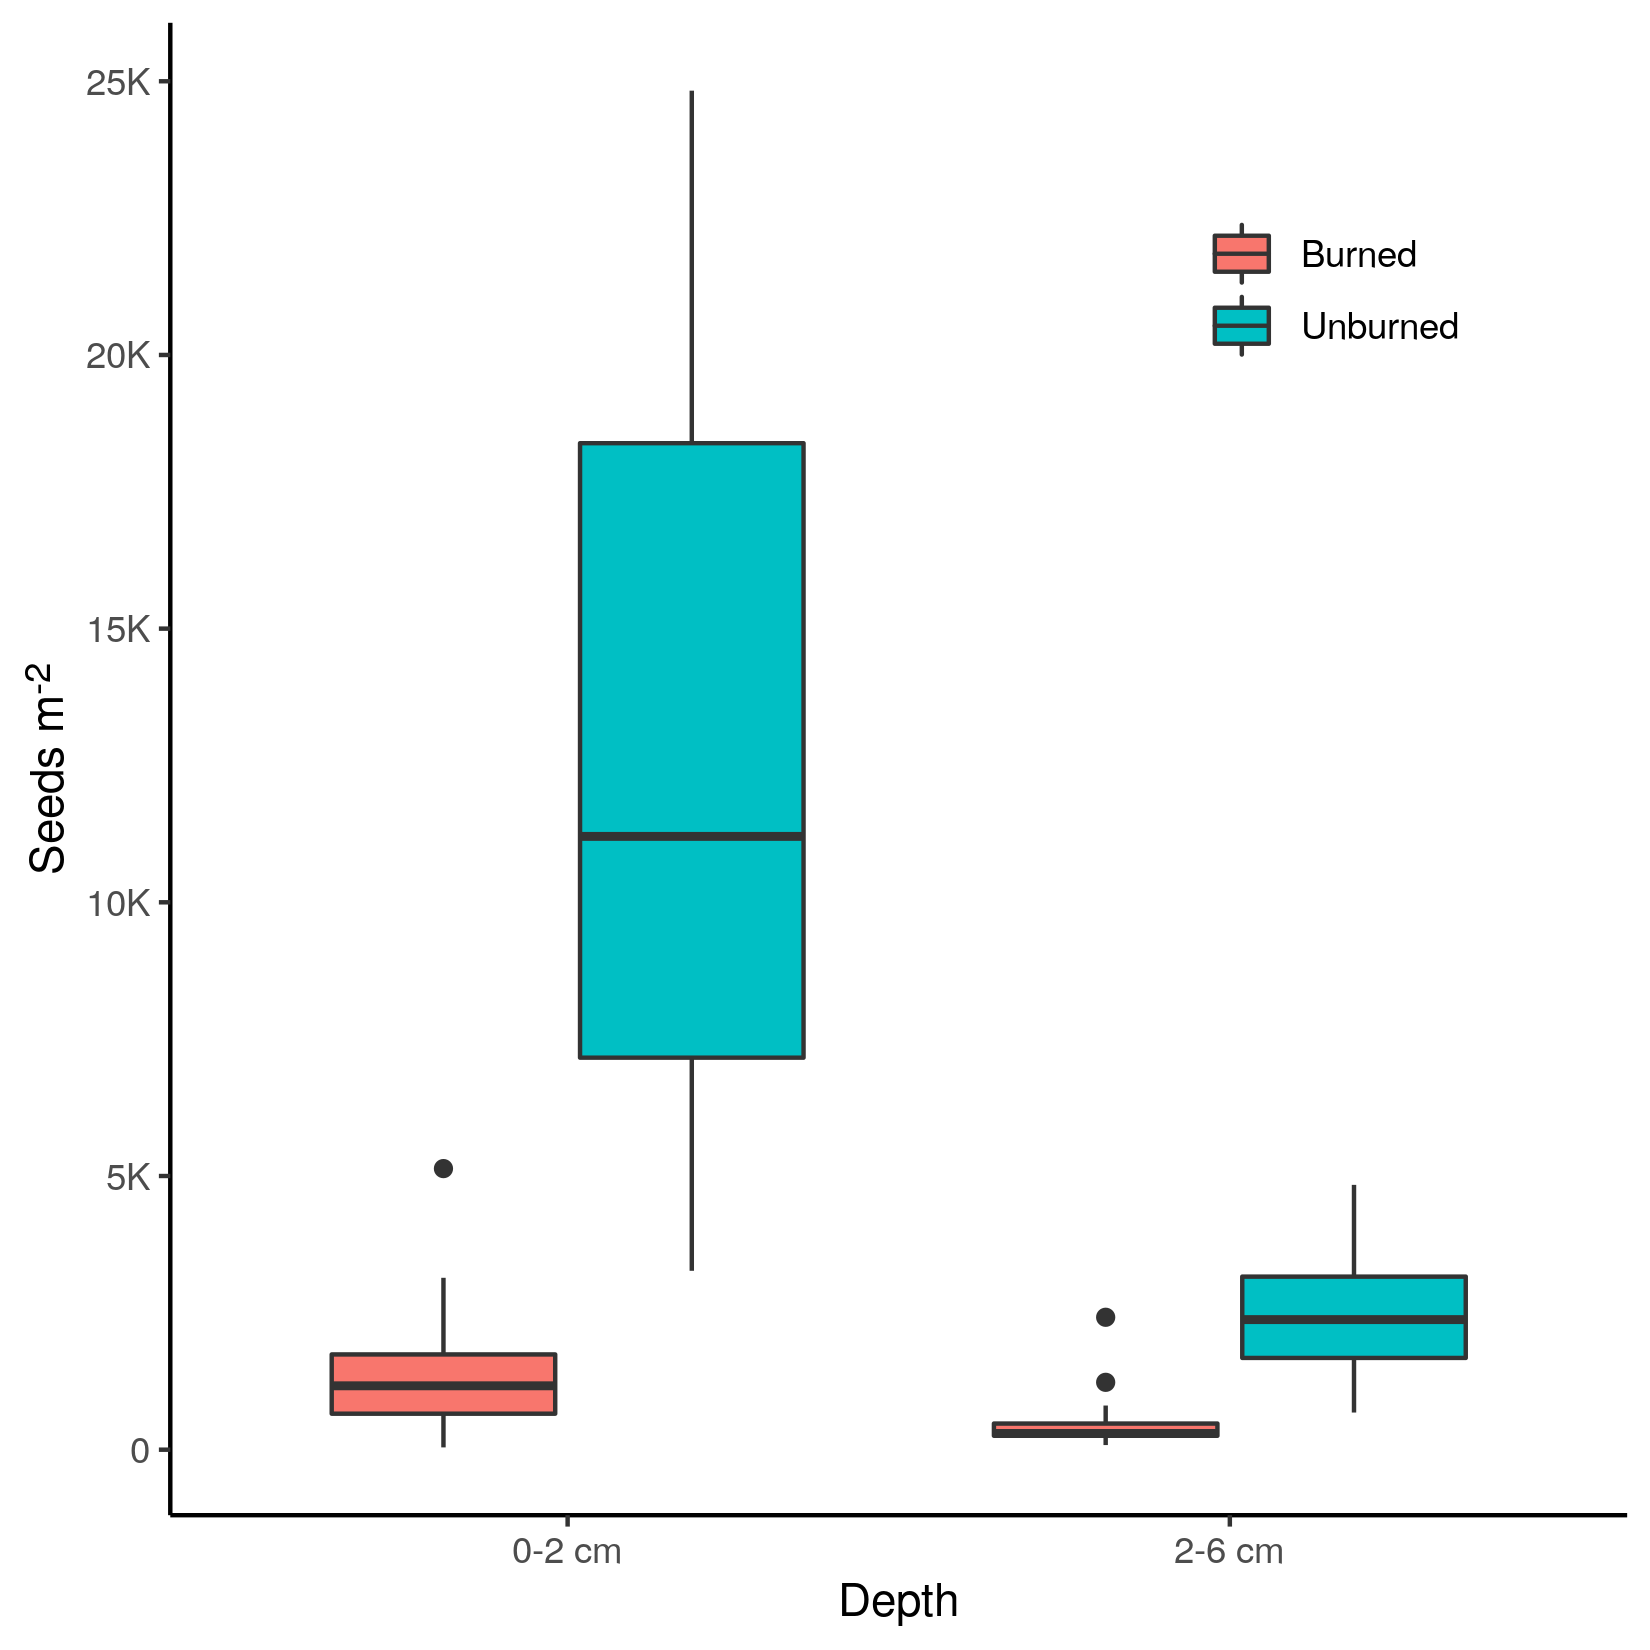
\includegraphics{images/depth_x_burned_counts.png}
\caption{Total seed counts per plot.}
\end{figure}

\newpage

\begin{figure}
\centering
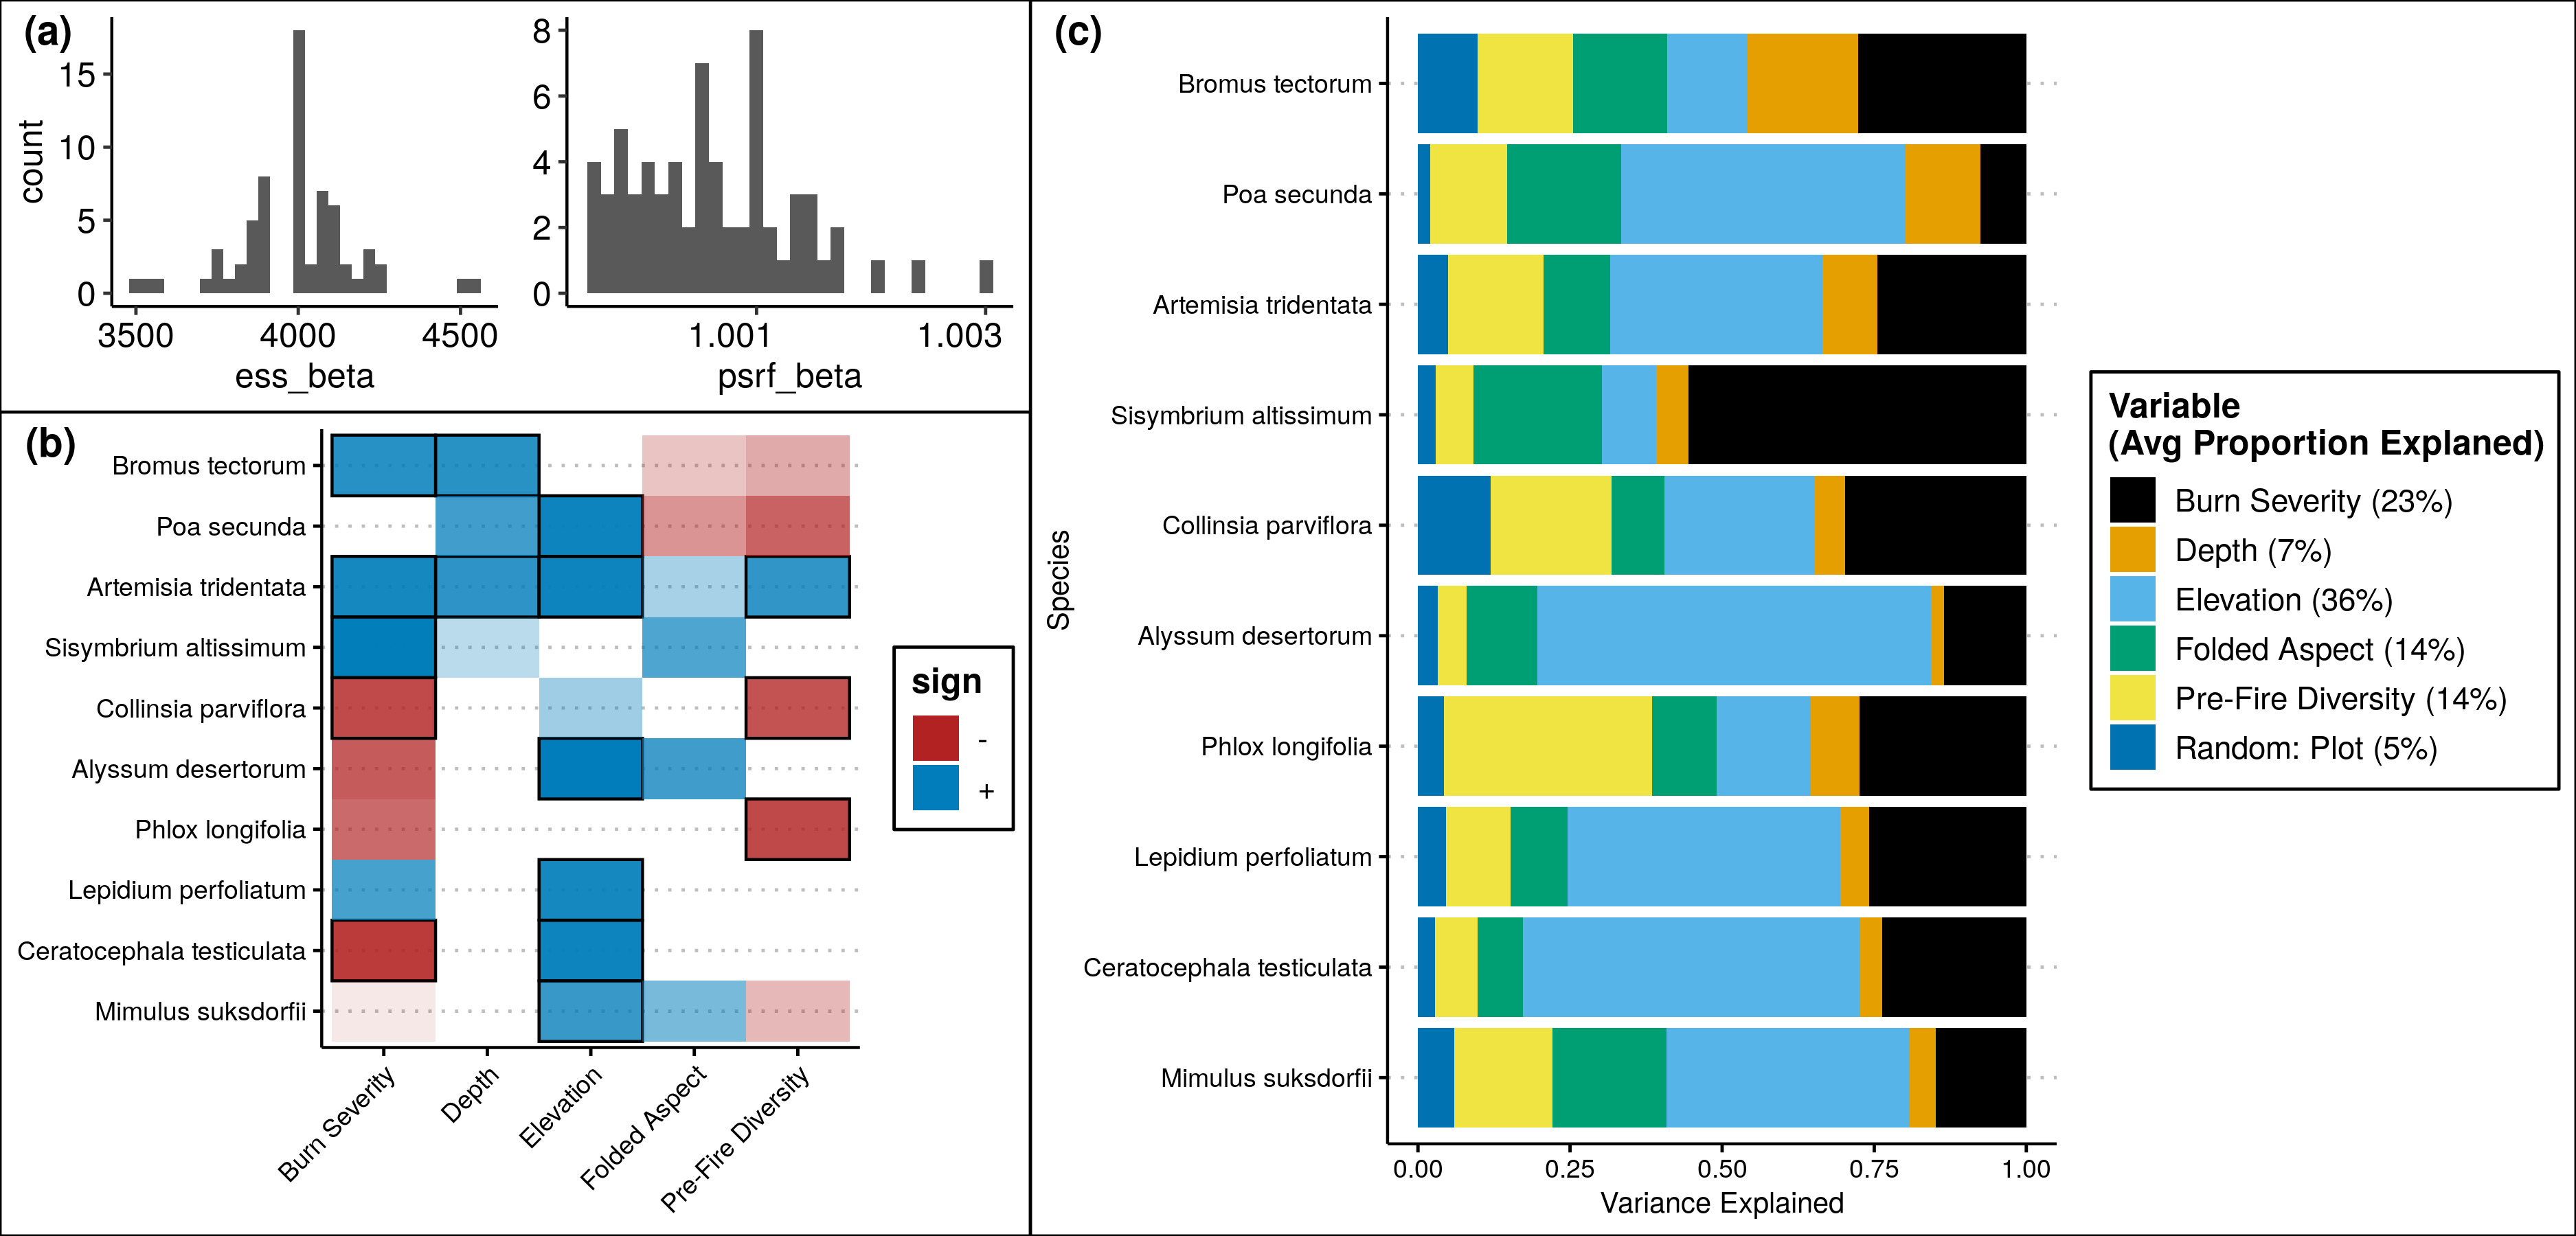
\includegraphics{images/jsdm_stuff.png}
\caption{a) Model convergence diagnostics. On the left is the effective
sample size after adjusting for autocorrelation (ideally 4,000), and on
the right is the Gelman diagnostic, ideally 1. b) Predictor variables
that had at least 80\% support. Variables with 95\% support are outlined
in black. The level of transparency corresponds to the level of support.
c) Variance partitioning by species. Average across all species per
variable is given in the legend. Species are ordered by prevalence.}
\end{figure}

\newpage

\begin{figure}
\centering
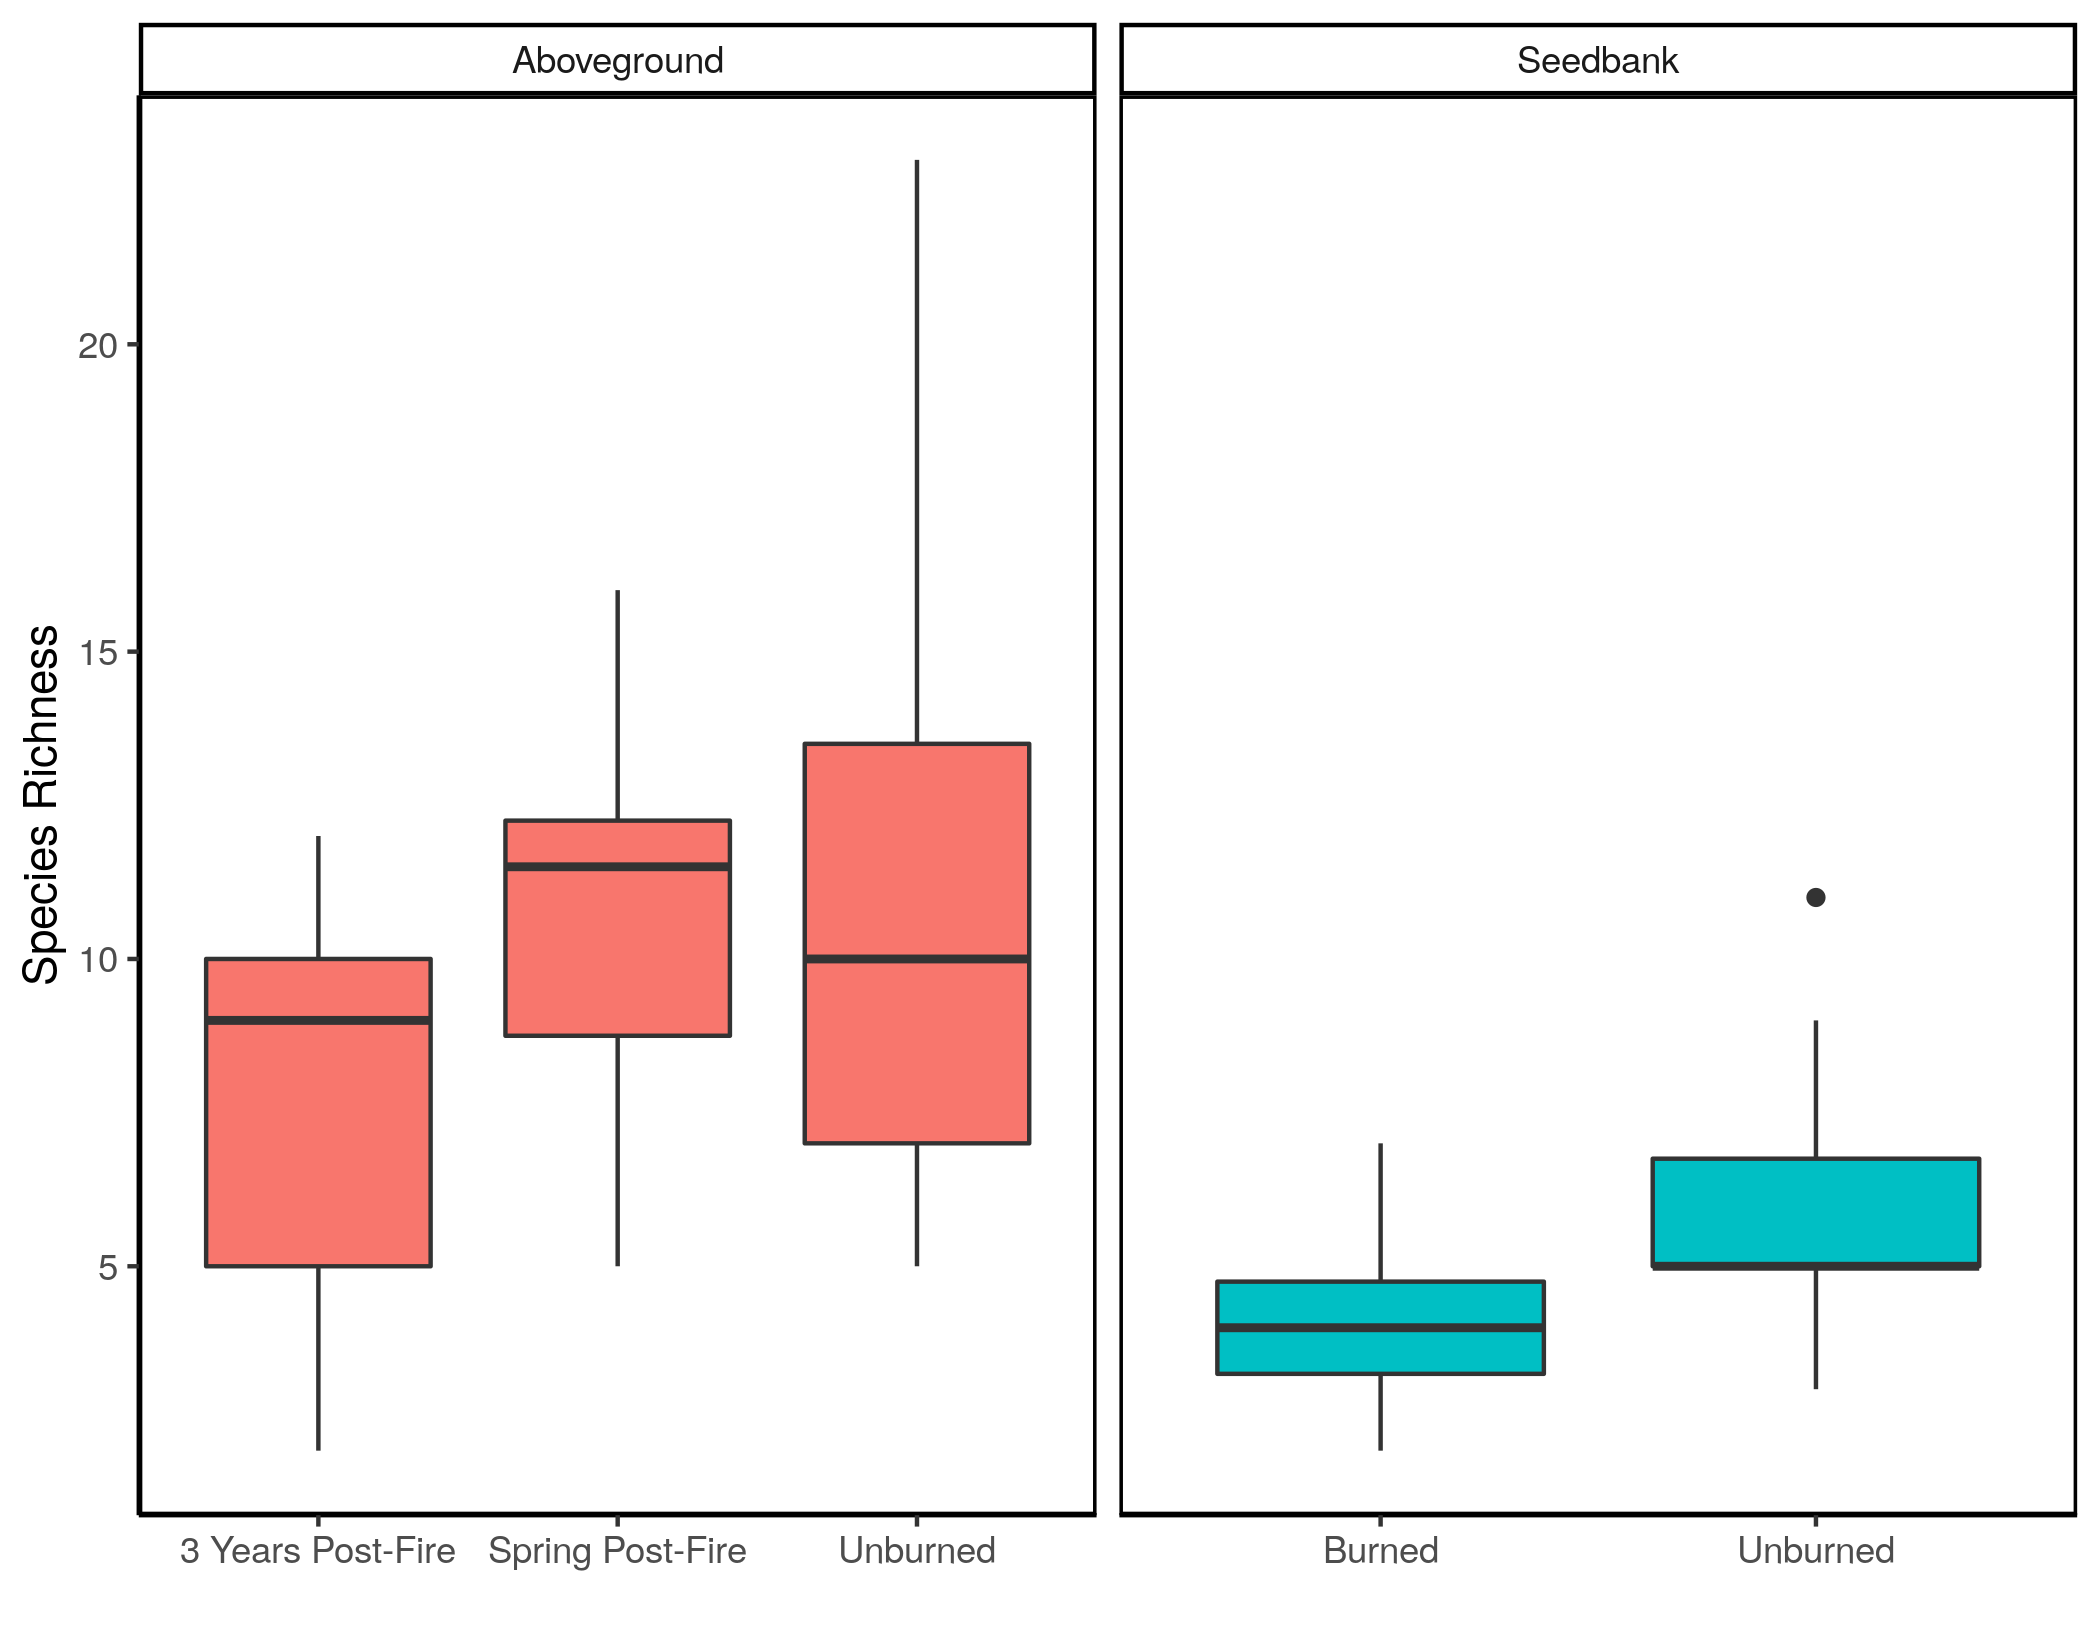
\includegraphics{images/richness_fig.png}
\caption{Species richness at different sampling times and locations.}
\end{figure}

\end{document}
